\section{Introduction}

We aim to establish a metric for assessing the efficacy of a model, denoted as $\mathcal{M}(\hat{\vartheta}_N)$, in representing a specific process, $y(t)$.
Given the complexities associated with finite $N$, we will focus our analysis on the more tractable scenario of large $N$ ($N \rightarrow \infty$).

\paragraph*{Small number of experiments}
In the scenario of a few experiments, each experiment yields a singular outcome for every considered time instant:
\[\mathcal{D}\left\{ \left( u(1,\bar{s}),y(1,\bar{s}) \right), \left( u(2,\bar{s}),y(2,\bar{s}) \right),\dots \right\}\]
Consequently, all predictors are contingent upon $\bar{s}$ independently at each prediction step, with the prediction error also being reliant on $\bar{s}$. 
When considering multiple experiments individually, divergent outcomes are obtained.

The points $\hat{\vartheta}_N(s)$ derived from each experiment constitute a collection of points. 
Consequently, this scenario presents challenges as it results in multiple valid minima points.

\paragraph*{Large number of experiments}
In the scenario where $N\rightarrow\infty$, multiple curves converge, leading to the emergence of a well-defined point.
Consequently, in this case, the cost function $J_N(\vartheta,s)$ converges to a single asymptotic curve, with the corresponding minima gradually approaching each other.

\begin{theorem}
    Under the given assumptions, as $N\rightarrow\infty$, we observe that:
    \[J_N(\vartheta,s)\rightarrow\hat{J}(\vartheta)=\mathbb{E}\left[\varepsilon(t,\vartheta,s)^2\right]\]
    Furthermore, defining $\Delta=\left\{ \vartheta^\ast: \bar{J}(\vartheta^\ast) \leq \bar{J}(\vartheta) \quad \forall\vartheta\right\}$ as the set of global minimum points of $\bar{J}(\varepsilon)$, it follows that:
    \[\hat{\vartheta}_N(s)\rightarrow \Delta\]
\end{theorem}
\begin{corollary}
    If $\Delta=\left\{ \vartheta^\ast \right\}$, i.e. $\bar{J}(\vartheta)$ possesses a unique minimum, then:
    \[\hat{\vartheta}_N(s)\rightarrow\vartheta^\ast\]
\end{corollary}

Our aim, considering the true model of the system $\mathcal{M}(\vartheta^\circ)$, is to converge towards $\hat{\vartheta}_N(s)\rightarrow\vartheta^\circ$. 
This equivalence suggests that $\vartheta^\circ \in \Delta$, if $\Delta=\left\{ \vartheta^\ast \right\}$, then $\vartheta^\circ=\vartheta^\ast$. 

To establish that $\vartheta^\circ \in \Delta$, we present the following theorem:
\begin{theorem}
    $\vartheta^\circ \in \Delta$
\end{theorem}
\begin{proof}
    Consider the prediction error for a generic $\vartheta$:
    \[\varepsilon(t,\vartheta)=y(t)-\hat{y}(t\mid t-1,\vartheta)\]
    By adding and subtracting the predictor for $\vartheta^\circ$, we obtain:
    \[\varepsilon(t,\vartheta)=\underbrace{y(t)+\hat{y}(t\mid t-1,\vartheta^\circ)}_e(t) - \hat{y}(t\mid t-1,\vartheta^\circ)-\hat{y}(t\mid t-1,\vartheta)\]
    The expected value of $\varepsilon(t,\vartheta)$ is then computed as follows:
    \begin{multline*}
        \mathbb{E}\left[ \varepsilon(t,\vartheta)^2 \right] = \underbrace{\mathbb{E}\left[ e(t)^2 \right]}_{\lambda^2}  + \mathbb{E}\left[ \left( \hat{y}(t\mid t-1,\vartheta^\circ)-\hat{y}(t\mid t-1,\vartheta) \right)^2 \right] +\\ +2\underbrace{\mathbb{E}\left[ e(t)\left( \hat{y}(t\mid t-1,\vartheta^\circ)-\hat{y}(t\mid t-1,\vartheta) \right)\right]}_0 
    \end{multline*}
    Consequently, we have:
    \[\mathbb{E}\left[ \varepsilon(t,\vartheta)^2 \right] = \lambda^2 + \mathbb{E}\left[ \left( \hat{y}(t\mid t-1,\vartheta^\circ)-\hat{y}(t\mid t-1,\vartheta) \right)^2 \right]\]
    Here, $\lambda^2$ is termed the unavoidable error term, independent of $\vartheta$. 
    On the other hand, the second term is $\vartheta$-dependent and is greater than or equal to zero. 
    Hence, it follows that:
    \[\bar{J}(\vartheta^\circ) \leq \bar{J}(\vartheta) \quad \forall\vartheta\]
    Therefore, if $J\in\mathcal{M}(\vartheta)$, then the parametric identification ensures that $\mathcal{M}(\hat{\vartheta}_N) \rightarrow \mathcal{S}$. 
\end{proof}

\subsection{Possible cases}
There exist four potential scenarios that may occur:
\begin{enumerate}
    \item $\mathcal{S} \in \mathcal{M}(\vartheta)$ and $\Delta$ is a singleton: 
        \[\mathcal{S}=\mathcal{M}(\vartheta^\circ)  \qquad \Delta=\left\{ \vartheta^\circ \right\}\]
        \begin{figure}[H]
            \centering
            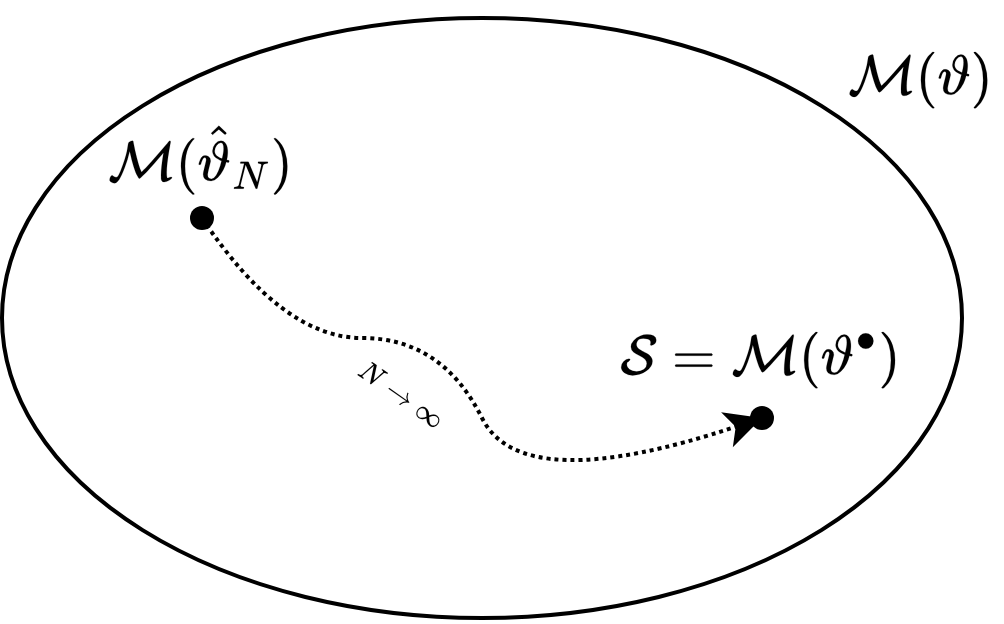
\includegraphics[width=0.4\linewidth]{images/one.png}
        \end{figure}
        As $N$ increases, we approach the correct model but only achieve a satisfactory approximation.
    \item $\mathcal{S} \in \mathcal{M}(\vartheta)$ and $\Delta$ is not a singleton:    
        \[\mathcal{S}\in\mathcal{M}(\vartheta^\circ)  \qquad \Delta=\left\{ \vartheta^\circ_1,\vartheta^\circ_2,\dots,\vartheta^\circ_n \right\}\]
        \begin{figure}[H]
            \centering
            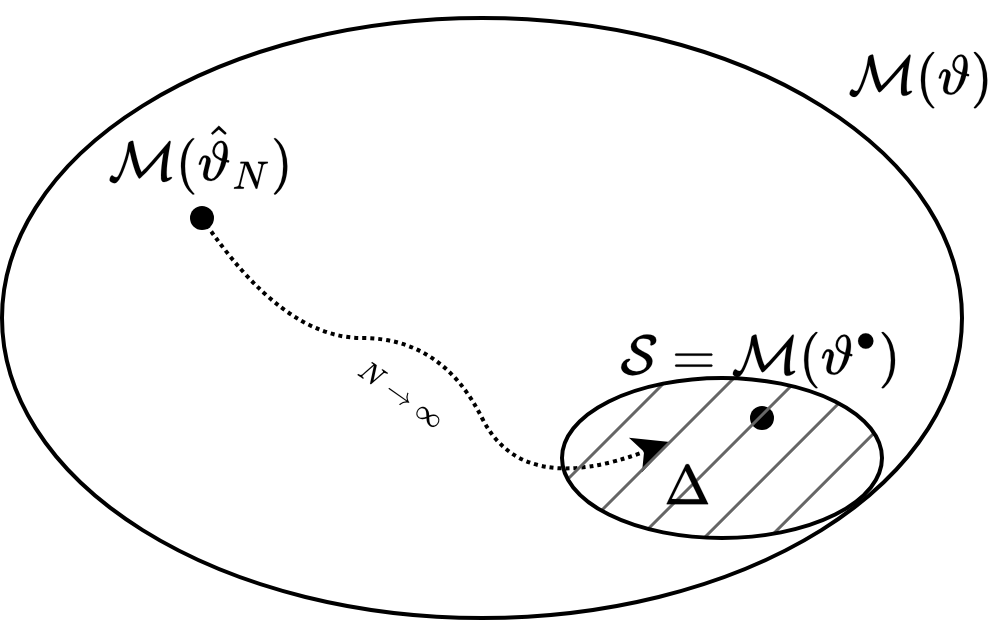
\includegraphics[width=0.4\linewidth]{images/two.png}
        \end{figure}
        With increasing $N$, we approach the set of global minima comprising the correct model, but with less precision compared to the first scenario.
    \item $\mathcal{S} \notin \mathcal{M}(\vartheta)$ and $\Delta$ is a singleton: 
        \[\mathcal{S}\notin\mathcal{M}(\vartheta^\circ)  \qquad \Delta=\left\{ \vartheta^\circ \right\}\]
        \begin{figure}[H]
            \centering
            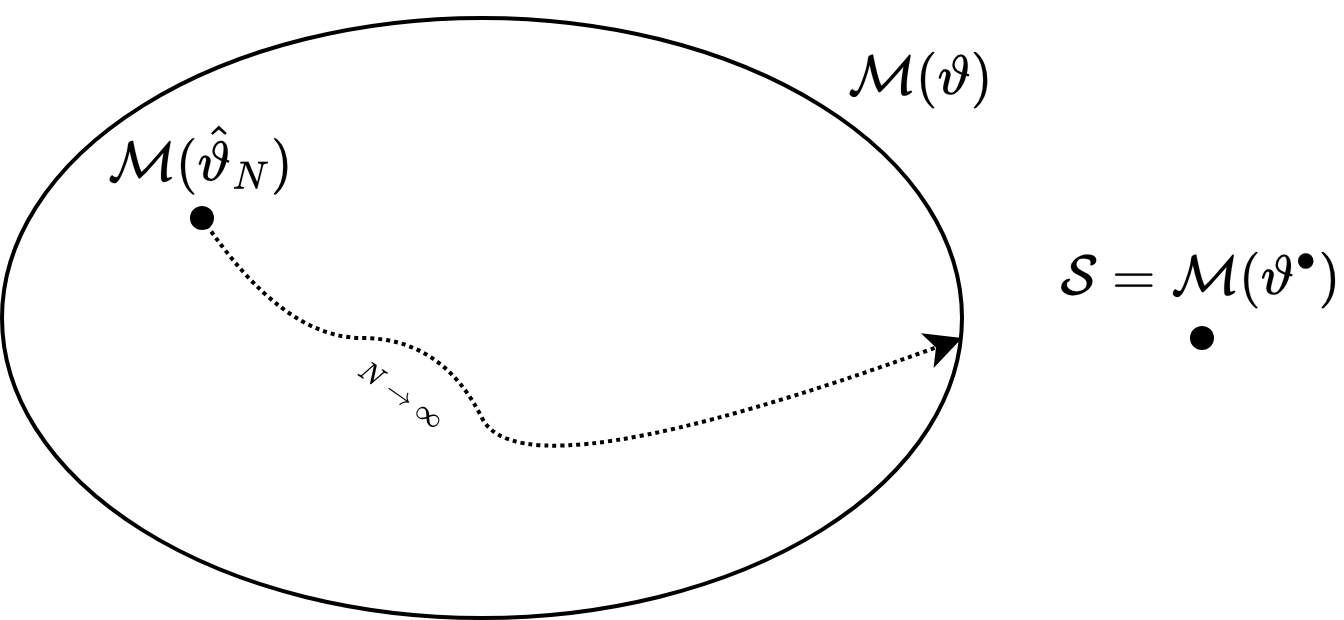
\includegraphics[width=0.55\linewidth]{images/three.png}
        \end{figure}
        As $N$ increases, we approach the correct model, but we are constrained by the limits of the considered set $\mathcal{M}(\vartheta^\circ)$. 
        Consequently, we obtain a result closest to correctness but not entirely accurate.
    \item $\mathcal{S} \notin \mathcal{M}(\vartheta)$ and $\Delta$ is not a singleton: 
        \[\mathcal{S}\notin\mathcal{M}(\vartheta^\circ)  \qquad \Delta=\left\{ \vartheta^\circ_1,\vartheta^\circ_2,\dots,\vartheta^\circ_n \right\}\]
        \begin{figure}[H]
            \centering
            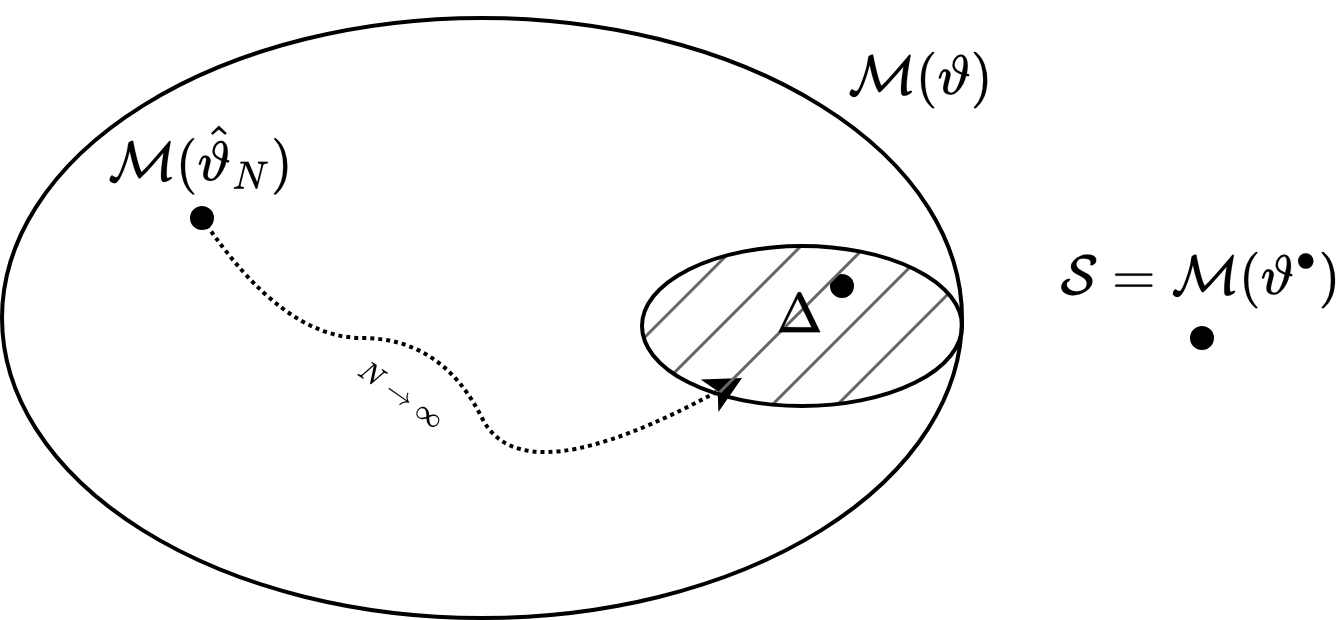
\includegraphics[width=0.55\linewidth]{images/four.png}
        \end{figure}
        With increasing $N$, we approach the set of global minima encompassing the correct model, albeit with less precision than the second scenario, as the set of points is contained within the model, but the sought-after model is not.
\end{enumerate}